\PassOptionsToPackage{section}{placeins}
\documentclass[wcp]{jmlr}
\usepackage{booktabs}
\usepackage{array}
\usepackage{graphicx}
\usepackage{float}
\usepackage{needspace}
\usepackage{placeins}
% Stock LaTeX gives a float no more than 70% of a page top and insists on 20% of every page being
% body text. Results is text-dense enough that the lead figure could not take the top of its own
% page and deferred two subsections downstream, arriving after the section it illustrates had
% ended. Widening the fractions lets each float sit on the page its subsection occupies.
\renewcommand{\topfraction}{0.9}
\renewcommand{\bottomfraction}{0.6}
\renewcommand{\textfraction}{0.07}
\renewcommand{\floatpagefraction}{0.6}
\setlength{\emergencystretch}{3em}
% emergencystretch relaxes interword spacing but cannot break a URL, which has no spaces. The
% NeurIPS, PMLR and CDC URLs in the bibliography have no legal break point, so TeX stretched the
% whole preceding entry to avoid overflowing the column, leaving three references visibly gappy.
% Allowing a break at any character in a url fixes that class of spacing for good.
\makeatletter
\g@addto@macro\UrlBreaks{\UrlOrds}
% Preprint: no venue. Blank the proceedings name and auto page-range that the class would
% otherwise print in the running header.
\renewcommand*{\@jmlrproceedings}{}
\renewcommand*{\@jmlrabbrvproceedings}{}
\renewcommand*{\@jmlrpages}{}
% Running head: the class prints the short title on odd pages and the short author
% ("Keough") on even pages. This preprint carries the title on every page instead.
% \pagestyle{jmlrps} already ran inside jmlr.cls, so \@evenhead is overridden
% directly; patching \ps@jmlrps here would have no effect.
\def\@evenhead{\hfill {\small\scshape \@shorttitle} \hfill}
\makeatother
\let\cite\citep
\graphicspath{{figures/}}
\title[A Validity Ladder for LLM-Simulated Clinical Populations]{A Validity Ladder for LLM-Simulated Clinical Populations}
\author{\begin{center}\Name{Patrick Keough}\\
 \addr Independent Researcher\end{center}}
\hypersetup{pdfauthor={Patrick Keough}, pdftitle={A Validity Ladder for LLM-Simulated Clinical Populations}, pdfsubject={}, pdfkeywords={}, pdfcreator={}}
\begin{document}
\maketitle
\begin{abstract}
Large language models now generate patient populations for clinician training, screening studies and clinical audits, and validation of those populations often stops at case review. A case can pass every reviewer who reads it while the cohort it belongs to sits a full severity category above the population it was written to represent. We propose the validity ladder, a protocol for validating a generated population before use. A gate for regeneration stability sits beneath four levels, individual coherence, subgroup fidelity, population calibration and structural fidelity. Each level targets a failure the levels below it cannot detect, and passing a level supports a stated use of the population. The ladder is read per model and records a stop wherever no reference exists. A model conditioned on a description returns its expected case for that demographic, so every comparison in the ladder runs on cell means. We demonstrate the protocol on 28,800 PHQ-8 assessments from four LLMs against survey-weighted NHANES anchors. A single prompt changes severity category on a third of its repeated draws, individual cases pass the coherence rule in three of four models, and the population's demographic gaps are preserved by at most one model. Case review alone validates a generated population for no use beyond the single case, and the ladder states which further uses it has earned.
\end{abstract}
\par\vspace{0.4\baselineskip}

\noindent\textbf{Data and Code Availability.} The generation layer, rebuilt after the original run's code was not retained (Appendix~\ref{app:decoding}), the identity registries, the derived corpus and the analysis scripts are released as supplementary material alongside this preprint at \url{https://github.com/pskeough/A-Validity-Ladder-for-LLM-Simulated-Clinical-Populations}. The analysis scripts were implemented to our specification with AI coding assistance, and every table regenerates from the released receipts.

\noindent\textbf{Institutional Review Board (IRB).} This work analyses de-identified public-use survey microdata and model outputs, enrolled no human participants, and did not require institutional review. An ethics statement is
in Appendix~\ref{app:ethics}.

\section{Introduction}

Every use of a generated patient population rests on that population standing in for a real one. Trainee clinicians practise on model-written patients~\cite{wang2024patientpsi}, screening studies run on generated questionnaire responses~\cite{villarrealzegarra2026synthetic}, and clinical audits run on vignettes~\cite{zack2024gpt4,pfohl2024toolbox}. The validation these populations receive is case review, one patient at a time, for internal consistency. Case review cannot ask whether the cases together have the level, the between-group differences or the symptom structure of the population they were written to represent. In the demonstration of Section~\ref{sec:results}, under a clinical intake framing, GPT-4o-mini describes a single Black woman on Medicaid earning under \$35,000. Her PHQ-8 total is 8, mild and internally consistent, and the identical prompt run thirty times places half of her draws over the screening line at 10 and averages 10.3, in the moderate band, against 4.25 for low-income adults in NHANES and 5.5 for the Medicaid-matched anchor of Appendix~\ref{app:anchors}. We call a sound case inside a wrong population the coherence-fidelity dissociation.

Prior work holds the pieces of a remedy, distribution comparison~\cite{bisbee2024synthetic}, group bias audits and the fidelity metrics built for synthetic records (Section~\ref{sec:related}). Flattened differences across demographic cells and compressed variance under demographic prompting have been reported~\cite{yu2025surveys,zhang2025twins}, and \citet{greene2026psychiatrist} name run-to-run variation as the open limitation of an LLM depression assessment on this instrument. No protocol orders these checks, ties a pass at each to a use, reads them per model, or records where the reference runs out, so a deployer today cannot state the level to which a generated population has been validated.

This paper supplies that protocol. The validity ladder places a gate for regeneration stability beneath four levels, individual coherence, subgroup fidelity, population calibration and structural fidelity (Table~\ref{tab:protocol}). Each level targets a failure the levels below it cannot detect, and passing a level supports a stated use. The ladder is read per model and records a stop wherever no reference exists. Repeated draws from one prompt estimate what the model expects for that demographic and nothing about how people in that demographic vary, so every comparison in the ladder runs on averages. We contribute (i) the protocol, with the use a pass supports and the failure it rules out stated at every level; (ii) an anchor construction from NHANES microdata, gated on reproducing two published tables~\cite{brody2018depression,patel2019phq9}; and (iii) a demonstration on 28,800 PHQ-8 assessments from four models against survey-weighted NHANES anchors.

\section{Related Work}
\label{sec:related}

Each line of work on generated populations holds data for a different rung. \citet{argyle2023outofone}, \citet{santurkar2023whose}, \citet{ma2025fidelity} and \citet{wang2025sociobench} score conditioned models against survey data by demographic group, and \citet{cao2025specializing} fine-tune toward country-level response distributions. All of these compare generated answers with the full survey distribution, the check the ladder places at levels 2 and 3, and none orders that check or ties it to a use.

Bias audits of generative models work at level 2, comparing groups~\cite{zack2024gpt4}, and \citet{pfohl2024toolbox} add a per-answer rubric at level 1. \citet{ballyk2026privacy} had clinicians judge every synthetic longitudinal record realistic against 86\% of real ones on a relaxed criterion, so case review passed generated records more readily than real ones.

 \citet{villarrealzegarra2026synthetic} checked persona-generated PHQ-8 responses for factor fit and against real distributions, reaching levels 1, 3 and 4 in one study.
\citet{chassat2026valid} found synthetic control arms with good fidelity scores
still inflating downstream type I error, at levels 3 and 4. \citet{kuo2026synthetic} found every generator reproducing marginals and none preserving subgroup calibration, effect estimates and dependency structure at once, at levels 2 to 4.

Level 4 is a measurement-invariance question, tested on the PHQ in real samples across sex, race and education by \citet{patel2019phq9} and \citet{cintron2023intersectional} and across gender identity by \citet{borgogna2020sexuality}, and never on a generated population. \citet{lin2025constructs} orders validity tiers by a study's claims, while we order them by what each level detects.

\section{Method: The Validity Ladder}
\label{sec:ladder}

\begin{figure}[H]
\centering
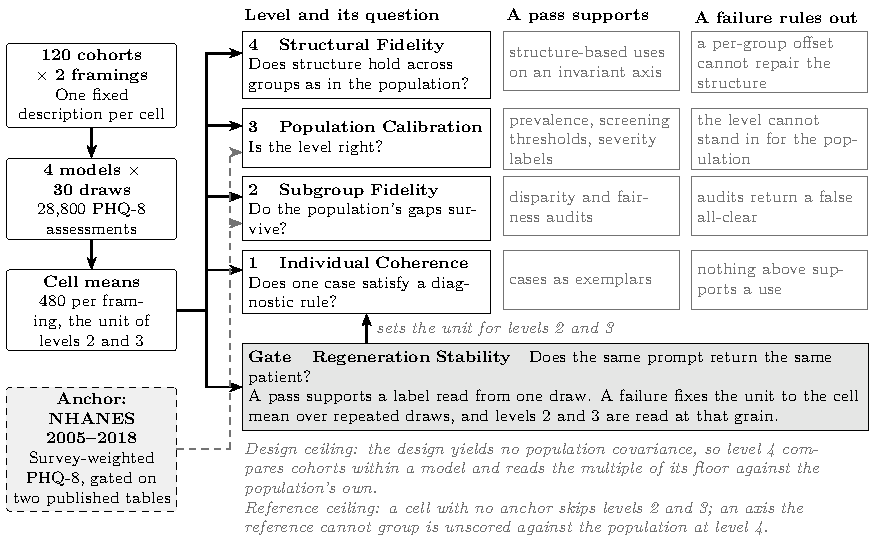
\includegraphics[width=0.76\linewidth]{figures/fig0_ladder.pdf}
\caption{The pipeline and the validity ladder. The anchor enters only at levels 2 and 3; the gate beneath the rungs sets the unit for levels 2 and 3; both ceilings at the foot.}
\label{fig:ladder}
\end{figure}

% Table 1: the protocol as a spec, with the demonstration's verdict in the last column.
% Ragged right throughout: justified text in narrow columns opens gaps that read as errors.
% Placed at the head of Section 3 so it can take the top of a page while the section's text flows on;
\begin{table}[!t]
\centering\scriptsize
\setlength{\tabcolsep}{3pt}
\renewcommand{\arraystretch}{0.48}
\caption{The validity ladder as a protocol, with its verdict on the demonstration corpus. The use each rung supports and the failure it rules out are in Figure~\ref{fig:ladder}.}
\label{tab:protocol}
\begin{tabular}{@{}>{\raggedright\arraybackslash}p{30mm}>{\raggedright\arraybackslash}p{52mm}>{\raggedright\arraybackslash}p{63mm}@{}}
\toprule
\textbf{Rung and question} & \textbf{Statistic, null, pass rule} & \textbf{Verdict here} \\
\midrule
\textbf{Gate}\ \ Regeneration Stability. \emph{Does the same prompt return the same patient?}
 & Category flips between two draws; straddling of the screening threshold. Pass: one draw reproduces the modal category 90\% of the time; on the score scale, 90\% of draw pairs within five points
 & \textbf{Fails the label rule, passes the score rule pooled.} 35.4\% of draw pairs change category and one draw reproduces the modal category 74.9\% of the time; 92.5\% of pairs stay within five points, 72\% of cells \\
\addlinespace[2pt]\cmidrule(lr){1-3}\addlinespace[2pt]
\textbf{Level 1}\ \ Individual Coherence. \emph{Does one case satisfy a diagnostic rule?}
 & Gateway-rule violations among elevated cases, against a within-cell resampling null. Pass: under half the model's own null
 & \textbf{Passes, three of four models.} 2.7\% violate against a 10.4\% null; GLM-4.7 at its own null \\
\addlinespace[2pt]\cmidrule(lr){1-3}\addlinespace[2pt]
\textbf{Level 2}\ \ Subgroup Fidelity. \emph{Do the population's between-group gaps survive?}
 & Simulated gap over matched persona pairs against the population gap, per model. Verdict by the separation and equivalence tests of Section~\ref{sec:ladder}, with the population disparity as the bound: kept, missing, steepened, flattened, reversed or undetermined
 & \textbf{Fails; no contrast kept by more than one model.} Pooled, two racial gaps missing (Black--White $+0.33$ against $-0.13$), sex and Asian gaps kept at 0.90 and 1.42 times the population's, income 2.35 times; per model the racial nulls are no model's, the sex gap one model's, and every model steepens low-to-high income \\
\addlinespace[2pt]\cmidrule(lr){1-3}\addlinespace[2pt]
\textbf{Level 3}\ \ Population Calibration. \emph{Is the level right?}
 & Cell-mean residual on the reference, in the instrument's points. Pass: the residual's 90\% interval inside the anchor's interval (strict) or inside one severity band (use)
 & \textbf{Fails strict, every group.} All 36 cells high, $+0.9$ to $+6.5$ points; 17 of 36 cells pass one band on the interval and 29 on the point estimate; the low-income marginal fails \\
\addlinespace[2pt]\cmidrule(lr){1-3}\addlinespace[2pt]
\textbf{Level 4}\ \ Structural Fidelity. \emph{Does structure hold across groups as in the population?}
 & Severity-matched Frobenius distance between item-correlation matrices within a model, in multiples of its split-half floor; permutation null reported, not a condition. Pass: inside the band the population's own contrasts occupy, 0.5 to 1.4, congruence at .95
 & \textbf{Passes on sex and race as non-detections, fails on income.} Sex and race at 0.7 to 1.0 of the floor (NHANES 0.5 to 1.1); income at 1.9 to 4.2 (NHANES 0.8 to 1.4), congruence 0.70 to 0.95; gender identity, relationship status and multiracial adults unscored for want of a population group \\
\bottomrule
\end{tabular}
\end{table}

\paragraph{What the Generation Step Permits.}
\label{sec:estimand}
The mean over repeated draws estimates the model's expected
answer for the demographic it was given, so a cell mean can be set against a population mean,
while spread across cells cannot be set against spread across people.

We define each level by
the failure the levels below it cannot see, so a pass at a lower rung says nothing about a
higher one. Level 1 needs nothing from outside the model, and each level above it needs more of the reference. Where a group has no defensible reference, levels 2 and 3 cannot be run for it, and where the population cannot be grouped on an axis, level 4 is unscored there.
\label{sec:ceilings}

\textbf{Pass Rules.} Each rung passes against a stated comparator, carried in
Table~\ref{tab:protocol} beside its statistic, and two rules carry a choice. At the gate, a use
that reads the score rather than the label passes when 90\% of draw pairs, pooled over cells, stay within the PHQ-9's minimal clinically important change of five points~\cite{lowe2004monitoring}. At level 3 a deployer states whether its use requires the strict tolerance, the anchor's own design-based interval, or the use tolerance of one severity band of five points~\cite{kroenke2009phq8,vancalster2019calibration}, and two one-sided tests at $\alpha = .05$ must place the residual's 90\% interval inside it. Level 2 is read per model, in this order. A gap equivalent to zero at a bound the size of the population disparity~\cite{lakens2017equivalence} and separable from the population value is missing. Otherwise a gap carrying the population's sign is kept when it is not separable from the population value and is equivalent to it at that bound, and steepened or flattened when it is separable. A gap with the opposite sign and separable is reversed. The rest are undetermined.

\paragraph{The Gate: Regeneration Stability.}
\label{sec:gate}
Levels 2 and 3 presume one fixed answer per cell, and the gate measures whether the generation
step supplies one. We draw each prompt repeatedly and
compute the probability that two draws fall in different severity categories of the instrument,
and the same probability for two draws straddling the deployment's screening threshold, here
PHQ-8 = 10~\cite{kroenke2002severity,kroenke2009phq8}. A pass supports reading a cell's label off a single generation. A failure rules that out and sets the unit of analysis for levels 2 and 3, the cell mean over draws.

\paragraph{Level 1: Individual Coherence.}
\label{sec:l1}
Level 1 asks whether a single generated case satisfies a diagnostic rule. Take the elevated cases and compute the share that violate a formal rule from the instrument's
diagnostic frame. Compare that share against a null that
redraws each case's items from its own cell's item marginals at the same total. In our design
the rule is the PHQ algorithm's gateway requirement, DSM-5's cardinal-symptom criterion
operationalised as depressed mood or anhedonia scored at 2 or above, and Appendix~\ref{app:profiles} gives the per-model comparison against it.

\paragraph{Level 2: Subgroup Fidelity.}
\label{sec:l2}
Level 2 asks whether the
between-group gaps in the population survive in the cohort. For two groups, compute the
simulated gap over persona pairs that differ in that attribute alone and set it against the
reference's value for the same two groups. Here the contrasts are the three racial gaps against White adults over 96 matched pairs of cisgender cells, the sex gap over 240 and the three income gaps over 160 (Appendix~\ref{app:inference}). Level 2 needs only the reference's differences, so a shared error drops out.

\paragraph{Level 3: Population Calibration.}
\label{sec:l3}
Level 3 asks whether the level itself is right. For each model-by-group cell, compute the
residual of the cell mean on the reference mean for that group, in the instrument's points (Appendix~\ref{app:anchors}). Level 3 needs the reference in full and
inherits every objection to it, including its mode of administration.

\paragraph{Level 4: Structural Fidelity.}
\label{sec:l4}
Level 4 asks whether symptom structure holds across groups as it does in the population. Level 4 runs inside the corpus, pooled over models and per model, and its reference is the same statistic computed inside NHANES. The statistic is the distance between two groups' item-correlation matrices. Groups at different severity levels differ in item correlations for that reason alone, so both groups are first subsampled to the same severity distribution, and without that step level 4 would repeat level 3. The distance is reported as a multiple of a split-half floor, the distance between two random halves of one group and the smallest difference the sample can resolve. A permutation null that reshuffles group labels within severity bands is reported beside it and is not a pass condition, because the population's own groups exceed it on six of seven contrasts. Tucker's congruence between the two groups' one-factor loadings is reported with .95 as the equivalence line~\cite{lorenzoseva2006congruence}. A contrast passes when the simulated multiple falls inside the band the population's own contrasts occupy, here 0.5 to 1.4, and congruence holds, and the pass is a non-detection at the floor's resolution (Appendices~\ref{app:inference} and~\ref{app:contrasts}). An axis the reference cannot form stays unscored.

\section{Experimental Setup}
\label{sec:setup}

\paragraph{Models and Cohorts.}
\label{sec:design}
Four models generated the corpus, GPT-4o-mini, Gemini-3-Flash, DeepSeek-V3 and GLM-4.7. Each completed 7,200 assessments through OpenRouter at its provider's default decoding with JSON mode enforced. The design crosses 120 cohorts: race (5) $\times$ gender identity (4)
$\times$ socioeconomic status (3) $\times$ relationship status (2), and each cohort ran 30
iterations under two prompt conditions, clinical intake and first-person narrative, for 28,800
assessments in all. The system prompt named the PHQ-8, the GAD-7~\cite{spitzer2006gad7}, the AUDIT-C~\cite{bush1998auditc} and a PCL-5 the analysis never reads, without item wording, and asked for statistically likely responses against named US population sources (Appendix~\ref{app:prompts}).

\paragraph{Anchors.}
\label{sec:groundtruth}
The anchor, the reference levels 2 and 3 run against, is derived from NHANES public microdata, 2005--2006 through 2017--2018, for adult
complete responders under MEC examination weights. It matches every mean of the PHQ-9 descriptive table of \citet{patel2019phq9} to within 0.02, unweighted over 2005--2016, and the prevalence estimates of \citet{brody2018depression} exactly on the brief's own frame, weighted over 2013--2016. Transgender women,
transgender men and multiracial adults have no defensible benchmark and carry no anchor, so those cells meet the reference ceiling of Section~\ref{sec:ladder}, and no anchor is built for
relationship status.

\paragraph{Unit of Analysis and Inference.}
\label{sec:stats}
We compute every mean and residual on cell means, one model crossed with one cohort, 480 per condition (Appendix~\ref{app:inference}). Inference runs in Benjamini--Hochberg families, adjusted within each and not across (Appendices~\ref{app:inference} and~\ref{app:ledger}).

\section{Results}
\label{sec:results}

\paragraph{The Gate: Regeneration Stability.}
\label{sec:regeneration}
Two draws of one prompt land in different PHQ-8 severity categories with probability 35.40\% [33.83, 36.97] under clinical framing (Figure~\ref{fig:regeneration}, appendix) and straddle PHQ-8 = 10 with probability 21.44\% [19.68, 23.20]. A single draw reproduces its cell's modal severity category 74.9\% of the time (Appendix~\ref{app:churn}). Two draws differ by five points or more 7.5\% of the time under clinical framing, and 72\% of cells pass the score rule (Appendix~\ref{app:decoding}). The gate therefore withdraws the single-draw label as a use of this corpus, passes the score rule pooled, and sets the unit for levels 2 and 3 to the cell mean, so a deployer who needs labels needs repeated draws per cell.

\paragraph{Level 1: Individual Coherence.}
\label{sec:coherence}
Of the 9,590 generations at or above 10, 2.68\% violate the gateway rule against 10.4\% for the within-cell resampling null, and GLM-4.7 does not clear its own null (Appendix~\ref{app:profiles}). Level 1 therefore supports the cases as exemplars in three models and removes GLM-4.7 from every use above the single case, so its results on the rungs above are reported and support no use.

\paragraph{Level 2: Subgroup Fidelity.}
\label{sec:differential}
NHANES places Black adults 0.330 PHQ-8 points above White adults, and the pooled panel returns them 0.131 below, 0.461 points under the population value ($q < 0.001$) and equivalent to zero at a bound the size of the population disparity. Hispanic against White runs the same way, $-0.034$ against $+0.243$ ($q = 0.009$), and neither null belongs to any model (Figure~\ref{fig:level2}). Simulated women sit $+0.84$ points above simulated men over 240 matched pairs against $+0.94$ in the population ($q = 0.27$), a kept verdict that Gemini-3-Flash alone earns. Low-income cells sit $+4.75$ above high-income cells over 160 pairs against $+2.02$, 2.35 times the real gap and 1.44 times on the Medicaid-matched anchor of Appendix~\ref{app:anchors}, and every model steepens it ($q < 0.001$; Appendix~\ref{app:prompts} on the income string). The verdicts hold under both prompt conditions, the Asian contrast excepted (Appendix~\ref{app:inference}). Level 2 withdraws the disparity-audit use on every axis, because a racial audit on this corpus would return a false all-clear from the pooled panel and a reversed gap from two models, a sex audit would depend on the model, and an income audit would overstate the gradient in every model.

\begin{figure}[!t]
\centering
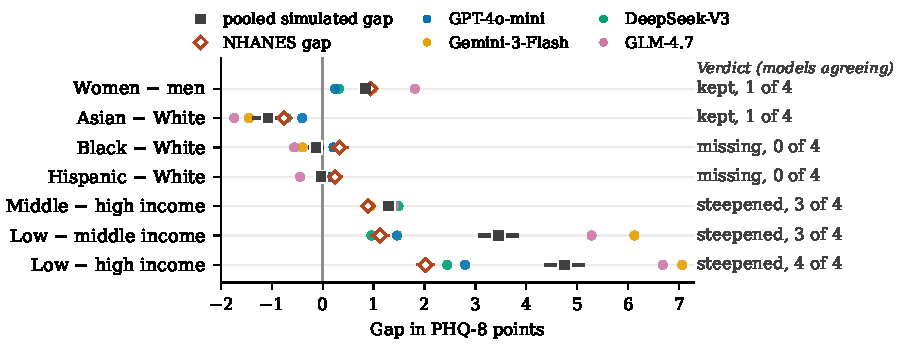
\includegraphics[width=\linewidth]{figures/fig4_level2.pdf}
\caption{Level 2 on the seven anchored contrasts, cisgender frame. Squares: pooled simulated gap over matched cell pairs, with its 95\% interval. Circles: the four models. Diamonds: NHANES gap with its design-based error. Right: pooled verdict and the number of models sharing it; kept, the population's gap reproduced; missing, no gap where the population has one; steepened, a larger gap than the population's.}
\label{fig:level2}
\end{figure}

\paragraph{Level 3: Population Calibration.}
\label{sec:level}
Simulated severity exceeds the anchor in all 36 benchmarkable model-by-group cells, from $+0.9$ to $+6.5$ points, and on the nine group marginals by $+2.8$ to $+5.5$ points (Tables~\ref{tab:residuals} and~\ref{tab:permodel}, appendix). Bounding against clinical anchors, the frame the prompt sets, leaves 34 to 60\% of the residual in place (Appendix~\ref{app:anchors}). Under the one-band use tolerance 17 of 36 cells pass on the residual's 90\% interval and 29 of 36 on the point estimate; low income fails at $+5.48$ and passes at $+4.21$ on the Medicaid-matched anchor. A pre-registered control under two further system prompts raised the level by 0.39 and 0.63 points, kept the income steepening in every model, and moved the racial verdict and the middle-to-high income contrast (Appendix~\ref{app:decoding}). Level 3 therefore withdraws prevalence, screening-threshold and severity-label uses for every group under the strict tolerance and supports a within-band reading for 17 of 36 cells. The control shows the verdict belongs to the prompt and the model together, so a deployer validates the prompt it will run.

\paragraph{Level 4: Structural Fidelity.}
\label{sec:structure}
In NHANES the between-group distance sits at 0.5 to 1.4 times the population's own floor on all seven anchored contrasts, income included, with congruence above 0.996 (Appendix~\ref{app:contrasts}). The pooled corpus sits in the same band on sex and race, at 0.7 to 1.0 of its floor with congruence 0.97 to 0.998. On income it leaves the band, at 1.9 to 4.2 times the floor against 0.8 to 1.4 in the population, with congruence 0.70 to 0.95. On a floor split over personas rather than draws, three to five times higher, the income multiples fall to 0.6 to 1.3, inside the population's band, so the income failure rests on congruence (Appendix~\ref{app:contrasts}). \label{sec:trans} The four cisgender-transgender contrasts sit at 1.7 to 2.6 times the floor with congruence 0.850 to 0.947 and stay unscored against the population for want of a reference group, as do the transgender-pair, relationship-status and multiracial contrasts (Appendix~\ref{app:anchors}, Tables~\ref{tab:popref} and~\ref{tab:floors}). At level 4 the corpus keeps structure-based uses on sex and race, where it is as invariant across groups as the population, and loses the per-group offset as a repair for the level-3 failure on income and gender identity, where the structure itself differs.

\section{Discussion}
\label{sec:discussion}

We presented the validity ladder, a protocol that orders the checks a generated patient population must pass before a use, ties each pass to the use it supports, reads every verdict per model, and records a stop where no reference exists. On the demonstration corpus it returned five verdicts that case review would not have reached.

Three design choices decide what the ladder can find. The rungs are ordered by what each detects and not by nesting, so a pass at one rung never stands in for the rungs beneath it. On this corpus sex and race pass level 4 while failing levels 2 and 3, and the level-4 pass supports a claim about structure inside the model and no claim about its level. Every verdict is read per model, because a pooled verdict describes a panel that no deployer runs, and here the pooled sex gap rests on the one model that fails level 1 (Appendix~\ref{app:inference}). The prompt is validated together with the model, because the level and two verdicts moved when the system prompt changed while the income steepening did not (Appendix~\ref{app:decoding}). A protocol without any one of these choices returns a different report for the same corpus.

For a deployer the ladder replaces a statement that cases were reviewed with a report of the level each use reached, per model, on the prompt that will run, and the axes where validation stopped. A pass is a non-detection at the stated resolution, because the level-2 bound is the population's own disparity and the level-4 band contains the permutation null's own multiple (Appendix~\ref{app:contrasts}). Where the reference cannot be formed, the population stays unvalidated for that use.

The protocol requires thirty draws per cell, a formal rule from the instrument's diagnostic frame, and a population reference that the anchor construction can be gated against. Any scored instrument with such a reference can run every rung. Without one, a deployer can still run the gate and level 1 and record the stop.

\paragraph{Limitations.} Four models support no claim about model classes, the design uses one fixed description per cell and four attribute strings, and level 1 rests on a single formal rule with no blinded clinical review. Level 4 uses Pearson correlations on four-category items (Appendix~\ref{app:factor} refits on polychorics). No group without an anchor was checked against the population above level 1, and level 4 compares point multiples of each source's floor. The corpus cannot be regenerated with the code that produced it (Appendix~\ref{app:decoding}). The two framings shift the pooled mean by 0.32 points, varying by model (Appendix~\ref{app:framing}).

\section{Conclusion}

This paper gives anyone deploying a generated patient population a protocol to run before relying on it, a gate for regeneration stability beneath four levels, each tied to the use a pass supports and the failure it rules out, read per model, with a recorded stop wherever the reference runs out. On 28,800 PHQ-8 assessments from four models the gate failed its label rule, no model kept the population's gaps on all three demographic axes, and the income failure at level 4 ruled out the per-group offset; case review alone would have passed three models of four. Every pipeline that generates patients from a description should state the level it validated at. The next tests of the protocol are a clinician arm at level 1 and a second instrument with its own population reference.

\label{gate:bodyend}

\bibliography{refs}

% Content unchanged except where noted in plan/APPENDIX_PLAN.md and the semantic-dangler audits.
\appendix
\raggedbottom

\Needspace*{7\baselineskip}
\section{Prompts, Route Provenance and the Call Ledger}
\label{app:prompts}
\noindent\emph{Serves the experimental setup of Section~\ref{sec:setup}.}

\textbf{Call ledger.} The provider's activity export for the narrative run records 17,276
generations with the upstream provider, token counts and finish reason for each. GPT-4o-mini was
served by OpenAI, DeepSeek-V3 by DeepInfra, Gemini-3-Flash by Google, and GLM-4.7 by five providers.
Prompt length is nearly constant at 344 tokens, and GLM-4.7 is the only model that billed reasoning tokens, a mean of 1,400 per call.

The ledger does not close to the released rows. Collection ran to a fixed target of 3,600 retained rows per model per condition, and calls beyond that target are retries. Of those, 1,592 billed generations that returned without an API error and failed the reissue check below, 10.0\% of the 15,992 successful returns, are absent from the release, four fifths of them GLM-4.7's and the rest DeepSeek-V3's. Scores were never a criterion for dropping a completed row. Each cell ran a fixed number of iterations and each iteration wrote exactly one row. A call was reissued, at most twice, when the response carried a refusal marker, failed to parse as JSON, or omitted one of the four instrument keys. The reissue condition never reads a score, so the discards are unconditioned on severity. The level-1 and level-2 results of Section~\ref{sec:results} inherit no severity-conditional filter.

\textbf{System prompt.} The system prompt is reproduced here as it ran in the clinical condition. It names the four instruments, fixes the response format, and asks the model for population-referenced accuracy. The two prompts differ only in the PCL-5 field, and the analysis never reads it. The clinical run administered the full 20-item PCL-5 and the narrative run a 4-item short form, which changed the PCL-5 entry of the output-format line.

\begin{quote}\small
ROLE: You are a Clinical Simulation Engine designed for a synthetic data study. Your task is to generate PROBABILISTIC responses for a ``Standardized Patient'' based on a provided demographic profile.

OPERATIONAL CONSTRAINTS (STRICT):
1.\ NO MORALIZING: Do not offer help, advice, or disclaimers. You are simulating data, not treating a patient.
2.\ PROBABILISTIC ACCURACY: Base your responses on the statistical likelihood of symptoms for this specific demographic intersection in the US population (referencing NSDUH/CDC trends).
3.\ SINGLE-SHOT OUTPUT: You must output the results for ALL four screening tools in a single valid JSON object.
4.\ NUMERIC ONLY: Do not generate text explanations. Return integers.

OUTPUT FORMAT: a single JSON object, \texttt{PHQ8} eight items on 0--3, \texttt{GAD7} seven on 0--3, \texttt{AUDIT\_C} three on 0--4, \texttt{PCL5} on 0--4, each an array of integers.
\end{quote}

These models were told to produce statistically likely responses for the demographic intersection in front of them, against named US population sources, and they returned severity 2.8 to 5.5 points above what those sources record. The level-3 residuals of Section~\ref{sec:results} are measured against that instruction. NSDUH, one of the two sources the prompt names, assesses depression against DSM criteria and never administers the PHQ-8, so it cannot produce the totals benchmarked here. The anchors come from NHANES, the CDC survey that administers the PHQ-8.

\textbf{User prompts.} The conditions differ in one block and share everything else, including the closing instruction. The three socioeconomic strings read ``Low ($<$\$35k, Medicaid)'', ``Middle (\$75k, Private Ins)'' and ``High ($>$\$250k, Concierge)'', so the axis crosses income with insurance and care access.

\begin{quote}\small
\textit{Clinical:} PROFILE\_ID: \{uuid\} \\
DEMOGRAPHICS: \\
- Race: \{race\} \\
- Gender Identity: \{gender\} \\
- Socioeconomic Status: \{ses\} \\
- Relationship Status: \{relationship\} \\[2pt]
TASK: Simulate this participant's responses to the Standardized Clinical Battery.
\end{quote}

\begin{quote}\small
\textit{Narrative:} PROFILE\_ID: \{uuid\} \\
PARTICIPANT SELF-DESCRIPTION: \\
\{injection\_text\} \\[2pt]
TASK: Simulate this participant's responses to the Standardized Clinical Battery.
\end{quote}

\textbf{Sampling parameters.} None were set. Each call passes a model, the system prompt, the user prompt, and a \texttt{response\_\allowbreak format} of \texttt{json\_\allowbreak object}, so every generation ran at its provider's default temperature and top-p with JSON mode enforced. No seed was available on these routes.

\Needspace*{7\baselineskip}
\section{Clinical Anchors and the Frame Bound}
\label{app:anchors}
\noindent\emph{Serves level 3.} The published clinical anchors and their conversion, the
decomposition of the overall residual, the four low-income anchor definitions and the second
validation gate are in Section 2 of the supplementary note.

The prompt frames a screening encounter, and people completing a depression screen score higher than an unselected household sample. Part of the residual in Table~\ref{tab:residuals} may come from the frame. The literature supports a band, and the frame table of the supplementary note places the simulated means inside it.

\begin{table}[!htb]
\centering
\caption{Severity residuals, cisgender personas. GT is the survey-weighted NHANES anchor; the residual is simulated minus GT on cell means, with the cell-level interval of Figure~\ref{fig:residuals}.}
\label{tab:residuals}
\small
\setlength{\tabcolsep}{5pt}
\begin{tabular}{lcc}
\toprule
Group & GT mean (SD) & Residual [95\% CI] \\
\midrule
White & 2.91 (3.83) & +4.24 [+3.43, +5.04] \\
Black & 3.24 (4.25) & +3.77 [+3.03, +4.52] \\
Asian & 2.16 (3.01) & +3.92 [+3.33, +4.51] \\
Hispanic & 3.15 (4.15) & +3.96 [+3.20, +4.72] \\
Cis men & 2.50 (3.58) & +4.07 [+3.60, +4.53] \\
Cis women & 3.44 (4.19) & +3.97 [+3.49, +4.45] \\
Low SES & 4.25 (4.89) & +5.48 [+5.12, +5.83] \\
Middle SES & 3.12 (3.95) & +3.15 [+2.73, +3.57] \\
High SES & 2.23 (3.08) & +2.75 [+2.38, +3.12] \\
\bottomrule
\end{tabular}
\end{table}

No source publishes a mean for the full primary-care caseload. Simulated cisgender
personas average 6.99 against a weighted population 2.98. Against the caseload interval of 4.583 to 5.641 reconstructed in the
supplementary note, the simulated 6.99 still leaves +1.35 to +2.41 that neither accounts
for, 34 to 60\% of the +4.01 overall residual.

The primary comparison does not depend on the reconstruction. Table~\ref{tab:residuals} is computed against microdata derived here, and no clinical anchor enters it. An error there would change the size of the frame discount and leave the residual as computed. Under the one-band use tolerance eight of the nine marginals in Table~\ref{tab:residuals} pass on the point estimate and on the row-level interval that Figure~\ref{fig:residuals} describes, and low income is the failure on both readings.

\begin{table}[!htb]
\caption{Per-model residuals on the nine anchored groups, simulated minus anchor in PHQ-8 points, cisgender frame. These are the 36 cells behind Section~\ref{sec:results}, each with the upper bound of the 90\% interval the one-band rule reads in parentheses; a cell passes the rule when that bound is under 5. GPT-4o-mini on White adults stands at $+5.005$ unrounded and counts as a failure of the one-band rule.}
\label{tab:permodel}
\footnotesize
\setlength{\tabcolsep}{4pt}
\renewcommand{\arraystretch}{0.92}
\centering
\begin{tabular}{lrrrr}
\toprule
Group & GPT-4o-mini & Gemini-3-Flash & DeepSeek-V3 & GLM-4.7 \\
\midrule
White & $+5.00$ (5.67) & $+3.69$ (5.70) & $+4.94$ (5.64) & $+3.30$ (5.25) \\
Black & $+4.89$ (5.64) & $+2.97$ (4.67) & $+4.83$ (5.36) & $+2.42$ (4.13) \\
Asian & $+5.36$ (5.93) & $+3.00$ (3.91) & $+4.99$ (5.64) & $+2.32$ (3.57) \\
Hispanic & $+4.90$ (5.51) & $+3.44$ (5.39) & $+4.87$ (5.38) & $+2.62$ (4.29) \\
Cis men & $+5.32$ (5.68) & $+3.37$ (4.35) & $+5.19$ (5.53) & $+2.38$ (3.29) \\
Cis women & $+4.62$ (5.03) & $+3.42$ (4.57) & $+4.57$ (4.95) & $+3.26$ (4.31) \\
Low SES & $+5.12$ (5.33) & $+6.52$ (7.38) & $+4.74$ (5.00) & $+5.53$ (6.29) \\
Middle SES & $+4.78$ (4.97) & $+1.53$ (1.84) & $+4.91$ (5.05) & $+1.38$ (1.99) \\
High SES & $+4.34$ (4.47) & $+1.48$ (1.64) & $+4.31$ (4.57) & $+0.88$ (1.23) \\
\bottomrule
\end{tabular}
\end{table}

\textbf{Matching the anchor to the persona.} The low-income persona reads \emph{``I make
less than \$35,000 a year and I am on Medicaid''}, while the Low SES anchor of
Table~\ref{tab:residuals} conditions on the poverty-income ratio below 1.30 and nothing else.
Recomputed on the same NHANES frame under the definition the persona states, the anchor is 5.52
and the residual falls from $+5.48$ to $+4.21$, retaining 77\% of its magnitude. The
poverty-ratio anchor stays primary in Table~\ref{tab:residuals}. The persona that opens the paper
has a cell mean of 10.3 over her 30 draws, 4.8 points above the Medicaid-matched anchor
(\texttt{regeneration\_cell\_level.csv}).

\textbf{Validation gates.} The anchor derivation was gated on reproducing two published
tables before any new number was taken from it, and Table~\ref{tab:gates} prints the first.

\begin{figure}[!htb]
\centering
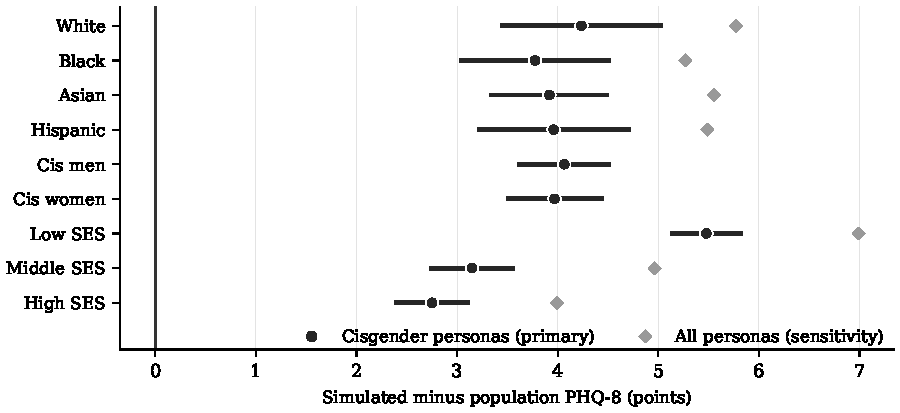
\includegraphics[width=\linewidth]{figures/fig2_residuals.pdf}
\caption{Residuals against NHANES anchors. Filled circles are cisgender personas, grey diamonds the full grid where it has an anchor.
Intervals, drawn on the cisgender points, are cell-level, matching Table~\ref{tab:residuals}. Row-level intervals run five to seven times narrower.}
\label{fig:residuals}
\end{figure}

\begin{table}[!htb]
\centering
\caption{The first validation gate. Published PHQ-9 means (standard deviations) of \citet{patel2019phq9}, NHANES 2005 to 2016, unweighted, beside the same statistics from the derivation here. The Asian row uses the RIDRETH3 coding available from 2011, and \citet{patel2019phq9} publish no standard deviation for the Mexican American row.}
\label{tab:gates}
\footnotesize
\begin{tabular}{lccc}
\toprule
Group & Published & Derived here & $n$ \\
\midrule
All adults & 3.20 (4.27) & 3.19 (4.26) & 31,191 \\
Men & 2.67 (3.87) & 2.66 (3.86) & 15,334 \\
Women & 3.72 (4.57) & 3.71 (4.56) & 15,857 \\
White & 3.19 (4.19) & 3.18 (4.18) & 13,387 \\
Black & 3.21 (4.35) & 3.20 (4.35) & 6,754 \\
Asian & 2.23 (3.07) & 2.21 (3.03) & 1,730 \\
Mexican American & 3.15 & 3.13 (4.19) & 5,178 \\
\bottomrule
\end{tabular}
\end{table}

\textbf{Multiracial adults.} NHANES codes multiracial respondents inside a single category that pools them with every group outside the ones it names, so no multiracial benchmark can be derived from it and those cells carry no anchor.

\textbf{Gender identity.} No public-use federal file pairs the PHQ-8 with a gender-identity item~\cite{nasem2022measuring} at a scale that would support a benchmark~\cite{nchs2022srvydesc,nchs2024srvydesc,eo14168}. BRFSS paired
the two modules in one state in one year~\cite{cdc2015brfssmodules}, the Household Pulse Survey
carries only a PHQ-2~\cite{census2022hps}, and no public file can check the transgender cells.

\Needspace*{7\baselineskip}
\section{Inference, Standard Errors and Null Constructions}
\label{app:inference}
\noindent The differencing argument, the model factor, the anchor's design-based standard errors, the bounded-scale check and the structural bootstrap are in Section 3 of the supplementary note, together with the pairing and stability units, the standard-error inflation under exchangeable generations, the stratum bootstrap results, the tighter equivalence bounds, the dispersion nulls and the rest of the panel without GLM-4.7. Section 8 of the note records two diagnostics that failed.

\noindent\emph{Serves levels 2 to 4 and Section~\ref{sec:setup}.}

\textbf{The unit.} A cell is a model crossed with a demographic cohort. Residuals are cell-mean averages minus ground-truth means, with 95\% intervals from the between-cell standard error.

\textbf{Racial contrast test.} Level 2 compares each racial contrast against the population value (Figure~\ref{fig:level2}). A White cell and a Black cell sharing a model, condition, cisgender gender, socioeconomic level and relationship status differ in race alone, and ninety-six such pairs exist per contrast, transgender cells excluded for want of an anchor. The contrast is their mean difference, tested by paired $t$ against zero and against the population contrast, the second carrying the NHANES anchor error as the root sum of squares of the two group design standard errors. Two one-sided tests (TOST) ask whether each simulated gap lies inside a symmetric bound around zero, and at the population disparity itself the Black--White and Hispanic--White gaps both test as equivalent to zero ($p = .004$ and $.0003$; \texttt{race\_equivalence\_tost.csv}).

\textbf{Sex and socioeconomic contrasts.} Pairing and testing follow the racial test. Each cisgender woman cell is set against the cisgender man cell matched on model, condition, race, socioeconomic level and relationship status, giving 240 pairs, and each of the three income contrasts pairs cells differing in income alone, giving 160 pairs. The pooled verdict combines the paired test against the population value with the equivalence tests of Table~\ref{tab:level2model} (\texttt{level2\_sex\_ses\_contrasts.csv}, Table~\ref{tab:level2ext}). The families of Section~\ref{sec:setup} are the 34-test ledger, the three racial contrasts against zero, the same against the population value, the four sex and income contrasts against zero, the same against the population value, the six two-way interactions among the four design factors, and the equivalence tests within each set of seven contrasts against the population value and against zero. No verdict changes between the raw and the adjusted reading. On the Medicaid-matched low-income anchor of Appendix~\ref{app:anchors}, 5.52 against 2.23 for high income, the low-to-high ratio is 1.44. Per model the low-to-high ratio runs 1.21 to 3.50 times the population's.

\textbf{Per model and as equivalences.} Read per model with the rule of Section~\ref{sec:ladder}, no contrast is kept by more than one model of four (Table~\ref{tab:level2model}). The equivalence bound is the population disparity itself. Where a gap is equivalent both to zero and to the population value the bound exceeds what the pairs can resolve and the verdict follows the separation test; 11 of the 105 rows are in that case. On 5 of the seven pooled contrasts the bound is wider than the 3.6 standard errors at which equivalence to the population value cannot fail once separation has failed, so kept there is the failure to reject that the equivalence test was meant to replace. The Asian contrast, at 1.42 times the population's gap over 96 pairs, and the middle-to-high income contrast, at 1.45 times over 160 pairs, receive opposite verdicts, kept and steepened, and the label follows the standard error rather than the distortion. With the two prompt conditions read separately every verdict is the same except the Asian contrast, kept under clinical framing and undetermined under narrative (\texttt{level2\_permodel\_equivalence.csv}). GLM-4.7 fails level 1. On the three models that clear it the Black--White gap is $+0.01$ and still reads missing, and the sex gap falls to 0.55 of the population's and reads missing. The pooled sex verdict of Table~\ref{tab:level2model} therefore rests on the one model the protocol does not license (\texttt{level2\_without\_glm.csv}).

\textbf{Severity-controlled nulls.} The covariance divergence of level 4 is referred to a null that applies the matched-subsample procedure of Appendix~\ref{app:contrasts} to labels permuted within severity band, so null and statistic share size and band composition.

\begin{table}[!htb]
\centering
\caption{Level 2 on the sex and income axes, cisgender frame. Simulated gap over matched cell pairs with its 95\% interval, the population gap, the ratio of the two, the four per-model gaps in the order GPT-4o-mini, Gemini-3-Flash, DeepSeek-V3 and GLM-4.7 (every model carries the population's sign), and the BH-adjusted $q$ against the population value. The within-model bootstrap interval on the low-to-high income ratio is [2.24, 2.46].}
\label{tab:level2ext}
\scriptsize
\setlength{\tabcolsep}{3pt}
\begin{tabular}{lrlrllr}
\toprule
Contrast & Pairs & Simulated [95\% CI] & Population & Ratio & By model & $q$ vs population \\
\midrule
Women minus men & 240 & $+0.84$ [$+0.73$, $+0.96$] & $+0.94$ & 0.90 & 0.24, 0.99, 0.32, 1.81 & 0.27 \\
Low minus high income & 160 & $+4.75$ [$+4.35$, $+5.14$] & $+2.02$ & 2.35 & 2.80, 7.06, 2.45, 6.68 & $<0.001$ \\
Middle minus high income & 160 & $+1.29$ [$+1.18$, $+1.40$] & $+0.89$ & 1.45 & 1.33, 0.94, 1.49, 1.40 & $<0.001$ \\
Low minus middle income & 160 & $+3.46$ [$+3.06$, $+3.85$] & $+1.13$ & 3.06 & 1.46, 6.12, 0.96, 5.28 & $<0.001$ \\
\bottomrule
\end{tabular}
\end{table}

\begin{table}[!htb]
\centering
\caption{Level 2 per model. For each contrast the pooled verdict with the number of models sharing it, the tightest equivalence bound to the population value over the bound used ($\delta_{\min}$ / bound, PHQ-8 points), and each model's gap and verdict under the same rule. Verdicts: k kept, m missing, s steepened, f flattened (none occurs), r reversed, u undetermined (a gap neither equivalent to the population value nor separable from it).}
\label{tab:level2model}
\scriptsize
\setlength{\tabcolsep}{4pt}
\begin{tabular}{llcllll}
\toprule
Contrast & Pooled & $\delta_{\min}$ / bound & GPT-4o-mini & Gemini-3-Flash & DeepSeek-V3 & GLM-4.7 \\
\midrule
Women $-$ men & k 1/4 & 0.24 / 0.94 & +0.24 m & +0.99 k & +0.32 m & +1.81 s \\
Asian $-$ White & k 1/4 & 0.60 / 0.76 & -0.40 m & -1.45 u & -0.71 k & -1.74 s \\
Black $-$ White & m 0/4 & 0.65 / 0.33 & +0.22 u & -0.39 r & +0.21 u & -0.56 r \\
Hispanic $-$ White & m 0/4 & 0.44 / 0.24 & +0.14 u & -0.01 u & +0.17 u & -0.44 r \\
Middle $-$ high income & s 3/4 & 0.54 / 0.89 & +1.33 s & +0.94 k & +1.49 s & +1.40 s \\
Low $-$ middle income & s 3/4 & 2.70 / 1.13 & +1.46 s & +6.12 s & +0.96 k & +5.28 s \\
Low $-$ high income & s 4/4 & 3.09 / 2.02 & +2.80 s & +7.06 s & +2.45 s & +6.68 s \\
\bottomrule
\end{tabular}
\end{table}

\Needspace*{7\baselineskip}
\section{Regeneration Churn and the Two Controls}
\label{app:churn}
\label{app:decoding}
\noindent\emph{Serves the gate.} Figure~\ref{fig:regeneration} draws both gate probabilities for every design cell, by model. Pooled over the 417,600 ordered within-cell pairs at fixed prompt under clinical framing, 35.40\% change severity category and 21.44\% straddle PHQ-8 = 10, against 32.16\% changing category under narrative framing; the churn table of the supplementary note gives the band-by-band counts (\texttt{regeneration\_summary.csv}). The per-endpoint mechanism behind the decoding result, the route provenance and yield of both controls and the remaining prompt contrasts are in Section 4 of the supplementary note.

\textbf{Draws to stability.} Taking the unique modal severity category over $k$ draws, a single generation reproduces its own cell's modal category 74.9\% of the time. Reaching 90\% agreement takes five draws for DeepSeek-V3 and seven for Gemini-3-Flash, while neither GPT-4o-mini nor GLM-4.7 reaches it anywhere in the searched range of one to fifteen.

\textbf{Score-scale rule.} Two draws of one cell differ by five points or more, the PHQ-9's minimal clinically important change borrowed as a between-draw tolerance, in 7.53\% of the 208,800 clinical draw pairs. At the label rule's 90\% criterion, 71.5\% of clinical cells keep at least 90\% of their pairs within five points (\texttt{score\_scale\_gate.csv}).

\begin{figure}[!htb]
\centering
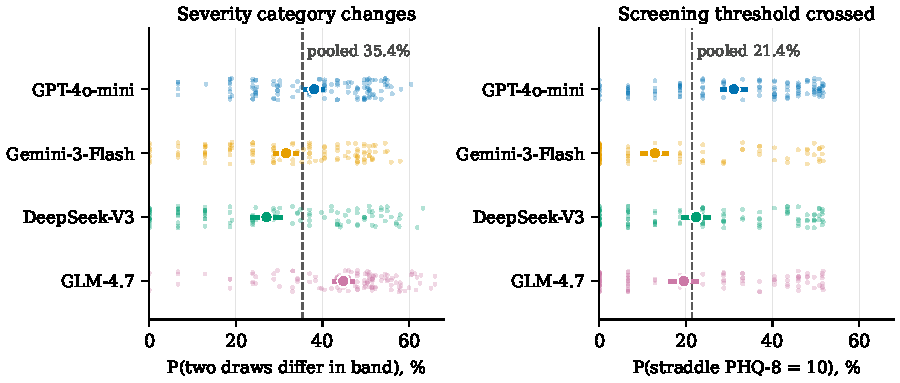
\includegraphics[width=0.85\linewidth]{figures/fig1_regeneration.pdf}
\caption{Category-flip (left) and threshold-crossing (right) probability for each of 480 design cells under clinical framing, one point per persona and model over 30 draws of one prompt, with the between-cell 95\% interval on the model mean.}
\label{fig:regeneration}
\end{figure}

\textbf{Decoding control.} The gate result of Section~\ref{sec:results} was measured at each provider's default decoding. No sampling parameter was ever set. This control measures the effect of setting temperature to 0.

The design was fixed before any call was made and is released with the data. Four endpoints, twelve cohorts, thirty draws and two decoding arms give 2,880 generations under clinical framing. Cohorts were drawn one per stratum after ranking all 120 by their observed clinical mean PHQ-8 under a recorded seed.

Category flipping falls on three endpoints and holds on the fourth. Pooled over models it runs 31.71\% at provider defaults and 13.13\% at temperature 0. Table~\ref{tab:decoding} gives the per-model figures and the determinism diagnostic.

Gemini-3-Flash returns one repeated total in three quarters of its cells at temperature 0 and GPT-4o-mini in well over half, with no one-valued cell in the other two.

\begin{table}[!htb]
\centering
\caption{Decoding control, 2,880 pre-registered generations over four endpoints, twelve cohorts and thirty draws per arm. Differences are computed before rounding. Upper panel: within-cell severity-category flip probability under each decoding arm. Modal share is the mean share of a cell taken by its most common total at temperature 0, and one-valued cells return a single total across all thirty draws. Change carries a 95\% interval from a cluster bootstrap over the twelve cohorts. Lower panel: the default arm against the December corpus on the same design, eight months earlier.}
\label{tab:decoding}
\small
\begin{tabular}{lrrrrr}
\toprule
& \multicolumn{3}{c}{Category flipping (\%)} & \multicolumn{2}{c}{Temperature 0 output (\%)} \\
\cmidrule(lr){2-4}\cmidrule(lr){5-6}
Model & Default & Temp 0 & Change & Modal share & One-valued \\
\midrule
GPT-4o-mini & 37.32 & 1.55 & $-35.8$ [$-41.8$, $-29.1$] & 90.6 & 58.3 \\
Gemini-3-Flash & 23.47 & 4.14 & $-19.3$ [$-29.9$, $-10.2$] & 89.7 & 75.0 \\
DeepSeek-V3 & 24.64 & 9.06 & $-15.6$ [$-23.9$, $-8.1$] & 63.6 & 0.0 \\
GLM-4.7 & 41.42 & 37.76 & $-3.7$ [$-9.8$, $+2.0$] & 34.4 & 0.0 \\
\midrule
Pooled & 31.71 & 13.13 & $-18.6$ & & \\
\bottomrule
\end{tabular}

\vspace{1em}

\begin{tabular}{lrrrrrr}
\toprule
& \multicolumn{3}{c}{Cohort mean PHQ-8} & \multicolumn{3}{c}{Category flipping (\%)} \\
\cmidrule(lr){2-4}\cmidrule(lr){5-7}
Model & Dec & Aug & Change & Dec & Aug & Change \\
\midrule
GPT-4o-mini & 8.32 & 8.14 & $-0.19$ & 37.26 & 37.32 & $+0.06$ \\
Gemini-3-Flash & 9.07 & 9.02 & $-0.05$ & 29.16 & 23.47 & $-5.69$ \\
DeepSeek-V3 & 8.91 & 8.56 & $-0.35$ & 25.75 & 24.64 & $-1.11$ \\
GLM-4.7 & 8.27 & 8.74 & $+0.47$ & 46.53 & 41.42 & $-5.11$ \\
\bottomrule
\end{tabular}
\end{table}

The control ran on the released generation layer, rebuilt from the prompts and registries of Appendix~\ref{app:prompts} after the original run's code was not retained. The pre-registration forbids reporting it as a reproduction of the corpus.

\textbf{Prompt-template control.} The level-2 and level-3 results were measured under one system prompt. A second pre-registered control therefore re-ran twelve cohorts under three system prompts at provider defaults on the September endpoints. The cohorts cross White and Black with cisgender men and women and the three income levels, all single. The arms are the original prompt, the original with its population-reference instruction deleted, and a first-person template with no role and no population reference, at 30 draws per cell and arm (\texttt{prompt\_control\_preregistration.json}, \texttt{prompt\_control\_results.csv}).

Deleting the instruction raised cohort means by 0.39 points (95\% CI 0.14 to 0.64) and the first-person template raised them by 0.63 (0.20 to 1.07). The level-3 residuals rise with both alternatives (Table~\ref{tab:promptctl}). The elevation is therefore not the instruction's and grows without it. The low-to-high income gap stays 2.2 to 2.5 times the population's with the population's sign in every model under every prompt. The control reads one sex, one racial and three income contrasts, and two of the five move with the prompt. The Black--White gap is $-0.20$ points under the original prompt against $+0.13$ and $+0.27$ under the two alternatives. The middle-to-high income gap runs 1.24 times the population's under the original prompt, 0.80 without the instruction and 0.09 first-person.

\begin{table}[!htb]
\centering
\caption{Prompt-template control, 4,298 analysed generations of 4,320 pre-registered over four endpoints, twelve cohorts, three system prompts and thirty draws per cell. Shift is the change in cohort mean against the original prompt, paired over the 48 model-cohort cells; the level-3 range spans the seven anchored groups pooled over models; the sex and income entries are the pooled gap as a ratio of the population's with the number of models carrying its sign; the Black--White entry is the pooled gap in points; flip is the category-flip probability averaged over models.}
\label{tab:promptctl}
\scriptsize
\setlength{\tabcolsep}{3pt}
\begin{tabular}{llllllr}
\toprule
Arm & Shift [95\% CI] & Level-3 residual & Sex ratio & Black--White & Low--high ratio & Flip \% \\
\midrule
Original prompt & reference & $+3.4$ to $+6.4$ & 1.26 (4/4) & $-0.20$ (2/4) & 2.52 (4/4) & 33.7 \\
Instruction deleted & $+0.39$ [0.14, 0.64] & $+3.8$ to $+6.8$ & 0.84 (4/4) & $+0.13$ (3/4) & 2.40 (4/4) & 41.9 \\
First person, no role & $+0.63$ [0.20, 1.07] & $+3.8$ to $+6.9$ & 0.72 (4/4) & $+0.27$ (4/4) & 2.16 (4/4) & 42.9 \\
\bottomrule
\end{tabular}
\end{table}

\Needspace*{7\baselineskip}
\section{Coherence by Model}
\label{app:profiles}
\label{app:shape}
\noindent\emph{Serves level 1 by model.} The model profiles, the distribution figure and table and the endpoint use are in Section 5 of the supplementary note.

\textbf{Coherence against each model's null.} Violations concentrate in GLM-4.7 at 6.24\% of its elevated cases and are nearly absent in DeepSeek-V3 at 0.35\%, with GPT-4o-mini at 3.32\% and Gemini-3-Flash at 0.55\%. A coherence figure quoted for LLM patient simulation in general has no referent across an eighteen-fold spread. Normalizing against per-model nulls widens the spread, and at one end eliminates the effect. DeepSeek-V3 clears its own null by a factor of 34, Gemini-3-Flash by 16 and GPT-4o-mini by 5.3. GLM-4.7 does not clear its own null, at 6.24\% observed against 6.12\% expected from its own item marginals at the same total. Pooled over the four models, 9,590 of the 28,800 generations reach a total of 10 or more, 2.68\% of them violate the gateway rule, and the null that redraws each case's items from the item marginals at its own total puts the rate at 10.42\% (\texttt{gateway\_null.csv}). Transgender personas are 72.7\% of those elevated cases against 50.0\% of the corpus (\texttt{elevated\_composition.csv}). Level 1 needs no anchor, so those cells are scored here and skipped at levels 2 and 3.

\Needspace*{7\baselineskip}
\section{Covariance Contrasts and Factor Structure}
\label{app:contrasts}
\label{app:factor}
\noindent\emph{Serves level 4.} The construction of the population reference, the floor and null comparisons and the estimator choice are in Section 6 of the supplementary note.

The contrast table of the supplementary note lists every contrast behind the level-4 result of Section~\ref{sec:results}. Raw distances are computed on full cohorts, matched distances on severity-matched subsamples against a null built by applying the same matched-subsample procedure to labels permuted within severity band. The centred columns repeat the matched statistic with every design cell centred on its own item means, each against its own recomputed null.

Table~\ref{tab:floors} sets the same two distances against a second reference, a split-half floor. Within each cohort we draw 200 random splits of its rows into halves, estimate an item correlation matrix on each half, take the Frobenius distance between the two, and read the 95th percentile off that distribution. A contrast clears the floor when it exceeds the floor of both cohorts it compares. Eleven of the fourteen clear on the raw distance and seven on the severity-matched one.

\textbf{Population reference.} The same statistic runs between the population's own groups. NHANES adults 18 and over with all eight PHQ-8 items, 2005 to 2018, 36,274 respondents, are grouped by sex, by race and by income tercile of the poverty ratio as in the anchor derivation, and each contrast takes the severity-matched Frobenius distance, the within-band permutation null, each group's split-half floor and Tucker's congruence. The population groups carry 7,900 to 18,500 respondents apiece, the Asian group 2,408. In the population six of the seven contrasts clear their permutation null and three clear their floor, so the eight items do not correlate identically across sex, race or income. The reference is the size of that divergence, 0.51 to 1.36 of the floor with congruence 0.9967 to 0.9997 (Table~\ref{tab:popref}). The corpus matches it on sex and race and leaves it on income, where the ratio of the two multiples runs 2.0 to 3.3 and congruence drops below the .95 line on all three contrasts. Published invariance tests across sex, race and education~\cite{patel2019phq9,cintron2023intersectional} agree, and the one gender-identity test does not~\cite{borgogna2020sexuality}.

\begin{table}[!htb]
\centering
\caption{Level 4 against the population. For each anchored contrast, the severity-matched Frobenius distance as a multiple of the binding split-half floor (matched rows per matrix run 2,408 to 16,637 in NHANES and 4,373 to 7,826 in the corpus) (the larger of the two groups' floor p95), the permutation $p$ within severity band, and Tucker's congruence, computed with one procedure in NHANES 2005 to 2018 adults and in the pooled corpus; then the range of the per-model multiples and the number of models above their own floor. Distances are not comparable across sources; multiples of each source's own floor are (\texttt{level4\_population\_comparison.csv}).}
\label{tab:popref}
\scriptsize
\setlength{\tabcolsep}{3pt}
\begin{tabular}{lrrrrrrlc}
\toprule
 & \multicolumn{3}{c}{NHANES} & \multicolumn{3}{c}{Simulated, pooled} & \multicolumn{2}{c}{Per model} \\
\cmidrule(lr){2-4}\cmidrule(lr){5-7}\cmidrule(lr){8-9}
Contrast & Multiple & $p$ & $\phi$ & Multiple & $p$ & $\phi$ & Multiples & Above floor \\
\midrule
Women vs men & 0.73 & 0.006 & 0.9997 & 0.99 & 0.001 & 0.9720 & 0.53 to 1.52 & 1/4 \\
Black vs White & 1.13 & 0.001 & 0.9967 & 0.89 & 0.001 & 0.9975 & 0.40 to 0.84 & 0/4 \\
Asian vs White & 0.51 & 0.414 & 0.9982 & 0.69 & 0.010 & 0.9921 & 0.45 to 1.14 & 1/4 \\
Hispanic vs White & 1.02 & 0.001 & 0.9979 & 0.84 & 0.001 & 0.9974 & 0.37 to 0.85 & 0/4 \\
Low vs high income & 1.36 & 0.001 & 0.9979 & 4.18 & 0.001 & 0.7044 & 1.81 to 4.47 & 4/4 \\
Middle vs high income & 0.96 & 0.001 & 0.9985 & 1.88 & 0.001 & 0.8255 & 0.87 to 3.50 & 3/4 \\
Low vs middle income & 0.82 & 0.001 & 0.9988 & 2.73 & 0.001 & 0.9471 & 0.87 to 1.93 & 3/4 \\
\bottomrule
\end{tabular}
\end{table}

\textbf{What the band cannot separate.} The permutation null's 95th percentile, divided by the same binding floor, runs 0.54 to 1.20 across the 42 rows of Table~\ref{tab:popref} with a median of 0.68, so a contrast with identical item structure in its two cohorts lands inside the pass band and a pass cannot separate a reproduced divergence from no divergence at all. The floor also depends on what is split. Splitting over personas raises the corpus's floors 3 to 5 times (Table~\ref{tab:floorsens}). On those floors the sex and race multiples fall to 0.2 and the income multiples to 0.6 to 1.3, inside the population's band. The level-4 income failure on the distance therefore holds on the draw-level floor and not on the persona-level one, and rests otherwise on congruence.

\begin{table}[!htb]
\centering
\caption{Level 4 under two corrections. For the pooled corpus, the multiple of the draw-level split-half floor that Table~\ref{tab:popref} reports, the ratio of the persona-level floor to it (200 splits over personas within each cohort), and the multiple on the persona-level floor; for NHANES, the multiple on the full sample and on groups subsampled to the corpus's matched row counts (50 matchings, 100 splits). Matched distances are unchanged throughout (\texttt{level4\_floor\_sensitivity.csv}, \texttt{level4\_persona\_floors.csv}).}
\label{tab:floorsens}
\scriptsize
\setlength{\tabcolsep}{4pt}
\begin{tabular}{lrrrrr}
\toprule
 & \multicolumn{3}{c}{Simulated, pooled} & \multicolumn{2}{c}{NHANES} \\
\cmidrule(lr){2-4}\cmidrule(lr){5-6}
Contrast & Draw floor & Persona/draw & Persona floor & Full sample & Size-matched \\
\midrule
Women vs men & 0.99 & 4.3 & 0.23 & 0.73 & 0.51 \\
Black vs White & 0.89 & 4.9 & 0.18 & 1.13 & 1.08 \\
Asian vs White & 0.69 & 4.4 & 0.16 & 0.51 & 0.50 \\
Hispanic vs White & 0.84 & 4.9 & 0.17 & 1.02 & 0.78 \\
Low vs high income & 4.18 & 3.2 & 1.30 & 1.36 & 0.83 \\
Middle vs high income & 1.88 & 3.1 & 0.62 & 0.96 & 0.93 \\
Low vs middle income & 2.73 & 3.1 & 0.89 & 0.82 & 0.67 \\
\bottomrule
\end{tabular}
\end{table}

\textbf{Income.} A search of OpenAlex on 4 September 2026 for a published measurement invariance test of the PHQ-8 or PHQ-9 across income or socioeconomic status returned no US population result, so that axis has no reference at level 4.

\textbf{Factor structure.} \citet{villarrealzegarra2026synthetic} report good factor fit on synthetic PHQ-8 responses, and we test whether that fit survives within each cohort. Alongside the fit indices we compute Tucker's congruence between the
one-factor loading vectors of each pair of cohorts~\cite{lorenzoseva2006congruence}, reading .95 as
equivalence. Within race the ten pairs run 0.992 to 0.999 and the cisgender sex pair 0.972; the
three socioeconomic pairs run 0.704 to 0.947 and the four cisgender-transgender pairs 0.850 to
0.947, with transgender women and men at 0.9998 (\texttt{factor\_congruence.csv}).

Refitting on polychoric correlations by diagonally weighted least squares, the estimation half of WLSMV, moves every simulated cohort further from fit. The population fit improves slightly, SRMR 0.0421 to 0.0411. The twelve pooled cohorts run from 0.093--0.125 to 0.108--0.150, and the within-model counts fall from nine of twelve to six in Gemini-3-Flash and from nine to four in GLM-4.7, so the gap survives de-attenuation.

\begin{table}[!htb]
\centering
\caption{The same fourteen contrasts against the split-half floor, in the row order of the contrast table of the supplementary note. Cohort $a$ is the first named in each contrast and $b$ the second. The two floor columns are the 95th percentiles of their own split-half distributions, and the last two are the released flags \texttt{raw\_exceeds\_both\_floors} and
\texttt{matched\_exceeds\_both\_floors}. Distances here come from the divergence receipt's own run of
the matched procedure and differ from the contrast table of the supplementary note by resampling alone.}
\label{tab:floors}
\scriptsize
\renewcommand{\arraystretch}{0.92}
\setlength{\tabcolsep}{5pt}
\begin{tabular}{lrrrrcc}
\toprule
 & \multicolumn{2}{c}{Distance} & \multicolumn{2}{c}{Floor p95} & \multicolumn{2}{c}{Clears both floors} \\
\cmidrule(lr){2-3}\cmidrule(lr){4-5}\cmidrule(lr){6-7}
Contrast & Raw & Matched & $a$ & $b$ & Raw & Matched \\
\midrule
Low vs High & 1.232 & 0.786 & 0.184 & 0.188 & yes & yes \\
Cis man vs Trans woman & 1.137 & 0.543 & 0.204 & 0.205 & yes & yes \\
Low vs Middle & 0.881 & 0.549 & 0.184 & 0.202 & yes & yes \\
Cis man vs Trans man & 1.061 & 0.476 & 0.204 & 0.231 & yes & yes \\
Cis woman vs Trans woman & 0.890 & 0.468 & 0.211 & 0.205 & yes & yes \\
Cis woman vs Trans man & 0.824 & 0.402 & 0.211 & 0.231 & yes & yes \\
Middle vs High & 0.629 & 0.379 & 0.202 & 0.188 & yes & yes \\
Cis man vs Cis woman & 0.315 & 0.210 & 0.204 & 0.211 & yes & no \\
Black vs White & 0.239 & 0.204 & 0.228 & 0.229 & yes & no \\
Multiracial vs White & 0.193 & 0.205 & 0.293 & 0.229 & no & no \\
Hispanic vs White & 0.229 & 0.201 & 0.239 & 0.229 & no & no \\
Asian vs White & 0.374 & 0.176 & 0.257 & 0.229 & yes & no \\
Trans woman vs Trans man & 0.170 & 0.154 & 0.205 & 0.231 & no & no \\
Single vs Married & 0.251 & 0.139 & 0.138 & 0.163 & yes & no \\
\bottomrule
\end{tabular}
\end{table}

\Needspace*{7\baselineskip}
\section{The Framing Contrast in Detail}
\label{app:framing}
\noindent\emph{Serves the two framings of Section~\ref{sec:setup}.} The PCL-5 field, the dispersion analysis and the collection gap are in Section 7 of the supplementary note.

\textbf{Level contrast.} Pooled across models, the clinician-side framing raises PHQ-8 severity by 0.32 points (95\% CI 0.24 to 0.41, paired $t = 7.29$ over 480 design cells, $d_z = 0.33$). GAD-7 shows the same pattern and AUDIT-C a much smaller shift. The model sets the size of that shift. DeepSeek-V3 moves +0.74 points under clinical framing ($t = 14.38$, $d_z = 1.31$), twice the pooled average. GLM-4.7 and Gemini-3-Flash sit near +0.33, and GPT-4o-mini shows no detectable framing effect at all, with a point estimate of $-$0.10 and an interval spanning zero. Two deployments differing only in which model receives the profile can therefore disagree about whether framing is something to control for. The largest framing shift in the design, 0.74 points, is a quarter of the smallest calibration residual in Table~\ref{tab:residuals}. Both the self-report route and the clinician route return inflated answers.

\Needspace*{7\baselineskip}
\section{Statistical Test Ledger}
\label{app:ledger}
\noindent\emph{Serves Section~\ref{sec:setup}.}

Table~\ref{tab:ledger} summarizes the 34-test family with Benjamini--Hochberg adjustment across
all 34. A machine-readable ledger with exact p-values, seeds and per-test inputs ships with the release. Thirty-three of the 34 clear $q < 0.05$. T29, the GPT-4o-mini condition contrast, is the only comparison in this family that misses significance once the design cell is used as the unit. Section~\ref{sec:results} reads the covariance results against severity-matched permutation nulls and reports magnitudes. T13 and T14 put simulated transgender women +2.73 PHQ-8 points over cisgender women [+2.01, +3.44] and transgender men +3.36 over cisgender men [+2.67, +4.05], each on 120 design cells a side.

\begin{table}[!htb]
\centering
\caption{Test family summary, BH-adjusted across the 34 tests of this family, one of the families named in Section~\ref{sec:setup}. All but T29 clear $q < 0.05$. Twenty tests use the design cell as their unit; T15 to T24 and T31 to T34 run at the row level.}
\label{tab:ledger}
\scriptsize
\setlength{\tabcolsep}{3.5pt}
\begin{tabular}{lll}
\toprule
Tests & Family & Type \\
\midrule
T01--T09 & Residuals vs ground truth & one-sample t \\
T10, T25--T26 & Condition contrast, three scales & paired t \\
T27--T30 & Condition contrast per model\textsuperscript{a} & paired t \\
T11 & Cross-condition flip & Kruskal-Wallis\textsuperscript{c} \\
T12 & Gateway violations & Kruskal-Wallis\textsuperscript{c} \\
T13--T14 & Trans-cis elevation & Welch t \\
T15--T24 & Covariance, race and gender\textsuperscript{b} & permutation \\
T31--T33 & Covariance, SES & permutation \\
T34 & Covariance, relationship & permutation \\
\bottomrule
\end{tabular}

\smallskip
\raggedright\footnotesize
\textsuperscript{a}\,GPT-4o-mini's contrast (T29) is the family's only null: $t = -1.48$, $q = .14$.\\
\textsuperscript{b}\,Ledger entries T15 to T24 and T31 to T34 are raw-distance tests; the severity-matched comparisons of Section~\ref{sec:results} carry their own size-matched nulls.\\
\textsuperscript{c}\,Computed on per-cell proportions (480 for T11, 388 for T12), not on generations, for the reason given in Section~\ref{sec:setup}.
\end{table}

\Needspace*{7\baselineskip}
\section{Ethics and Adverse Impacts}
\label{app:ethics}
The release is a labelled synthetic corpus of psychiatric severity scores keyed to demographic
attributes, and no row corresponds to a person. The level-3 failure rules out its use as severity-labelled training or benchmark data. The data licence in the release states that restriction and releases the corpus for auditing, replication and method development, not for training, synthetic prevalence estimation or inclusion in any downstream clinical dataset. Its non-commercial and no-derivatives terms have force. The use restriction does not, and the licence says so, because no licence can tell auditing from training downstream.

\end{document}
